\documentclass[a4paper]{article}
\usepackage[utf8]{inputenc}
\usepackage[margin=1in, footskip=0.25in]{geometry}

\usepackage{booktabs}
\usepackage{graphicx}
\graphicspath{../plots}

\usepackage{hyperref}
\usepackage[backend=bibtex, style=numeric, sorting=none]{biblatex}
\bibliography{references}

\usepackage[font=footnotesize,labelfont=bf]{caption}
\captionsetup{width=\linewidth}
\usepackage{subcaption}

\usepackage{listings}
\renewcommand{\lstlistingname}{Code}

\usepackage{xcolor}
\definecolor{backcolour}{RGB}{239,235,230}
\definecolor{lightgray}{gray}{0.7}
\lstdefinestyle{matlabcode}{
	language		=Matlab,
	backgroundcolor	=\color{backcolour},
	basicstyle		=\ttfamily\footnotesize,
	commentstyle	=\color{lightgray},
	numbers			=left,                    
	numbersep		=5pt,
	tabsize			=4,
	showstringspaces=false,
	frame			=leftline,
	captionpos 		= b
}
\lstset{style=matlabcode}

\usepackage{amsmath}
\usepackage{enumitem}


\begin{document}
	
	% ======================= start titlepage ==============================================
	
	\begin{titlepage}
		\begin{center}
			\Large Numerical Methods in Astrophysics \\
			\vspace{1cm}
			\huge{
				Project 3 \\
				\vspace{0.5cm}
				\textbf{Two Dimensional Random Walk,}\\
				\textbf{Circular Binary and} \\
				\textbf{Hypervelocity Stars} \\
				\vspace{1cm}
			}
			\Large \emph{Saksham Kaushal}
		\end{center}
	\end{titlepage}
	
	% =========================end titlepage ================================================
	
	\tableofcontents
	\newpage
	
	% ========================= Problem 1 ===================================================
	
	\part{Two Dimensional Random Walk} \label{problem1}
	
		% ------------------------------- Introduction --------------------------------------
		
		\section{Introduction} \label{1:introduction}
		
		A random walk is a process that describes the path of an object in a two dimensional plane consisting of successive random steps. In physics, these processes play an important role in study of polymers, Brownian motion, diffusion, etc. 
		
		% -------------------------------- Methods, Results ---------------------------------
		
		\section{Methods, Results and Discussions} \label{1:methods_results}
		
		\begin{figure} [h]
			\begin{subfigure} {.475\columnwidth}
				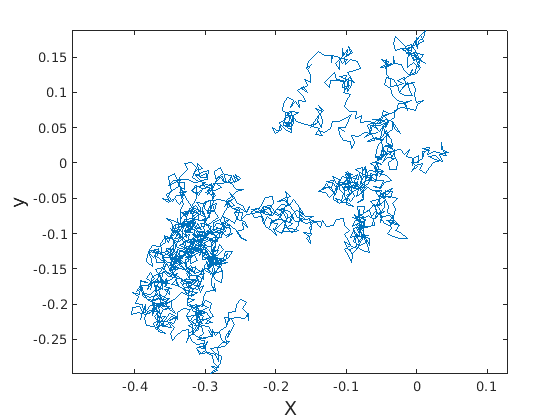
\includegraphics[width=\columnwidth]{../plots/1aa_randomwalk.png}
				\caption{Two dimensional random walk of a particle over 2000 time steps}
				\label{fig:1a}
			\end{subfigure}%
			\hfill
			\begin{subfigure} {.475\columnwidth}
				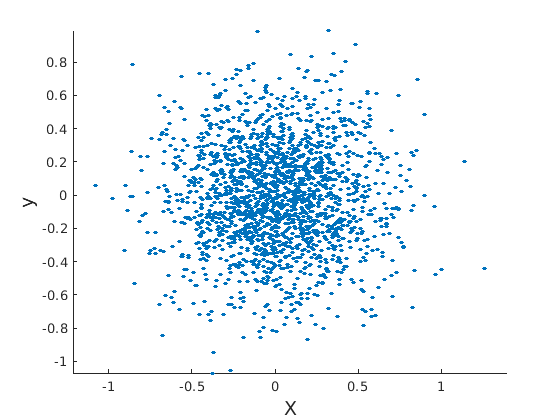
\includegraphics[width=\columnwidth]{../plots/1ab_randomwalk.png}
				\caption{Distribution of final coordinates of 2000 random walk particles}
				\label{fig:1b}
			\end{subfigure}
			
			\begin{subfigure} {.475\columnwidth}
				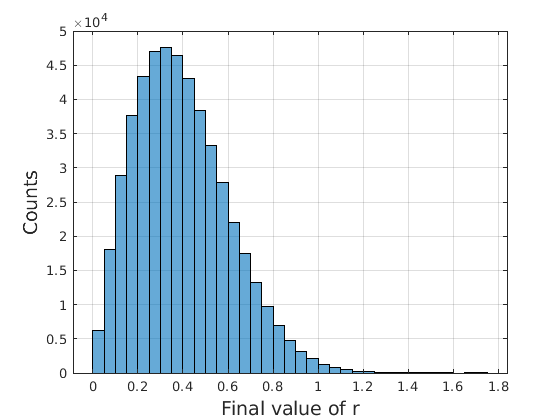
\includegraphics[width=\columnwidth]{../plots/1ac_hist_randomwalk.png}
				\caption{Number distribution with distance of \(5 \times 10^5\) random walk particles}
				\label{fig:1c}
			\end{subfigure}%
			\hfill
			\begin{subfigure} {.475\columnwidth}
				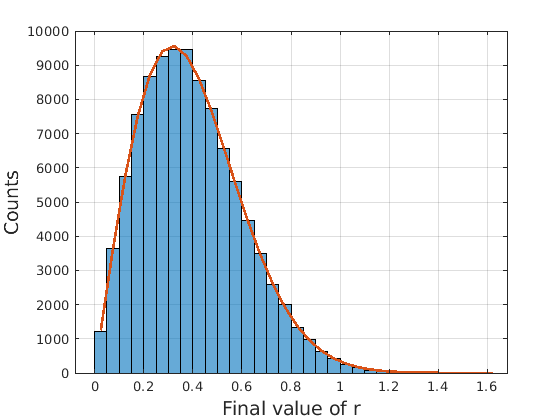
\includegraphics[width=\columnwidth]{../plots/1ad_hist_randomwalk.png}
				\caption{Theoretical estimates and observed distribution of \(10^5\) random walk points. The blue histogram represents the observed number distribution , while the red line is a plot of analytical estimates.}
				\label{fig:1d}
			\end{subfigure}
			\caption{Problem 1.1}
			\label{fig:1}
		\end{figure}
		
		\begin{enumerate} [label*=\textbf{(\alph*)}]
			
			% ---------------------------------- (a) ---------------------------------------------
			
			\item 
				\subitem \textbf{Methods  --} 
					Random walk of a particle which is initially located at origin (0,0), is computed for 2000 time steps. At each time step, the object moves a distance, \(d=0.01\) units in a random direction which is mathematically represented using angle, \(\theta \in [0,2\pi]\), computed in the Matlab program with the help of inbuilt function, \texttt{rand()}. This function generates random number uniformly in the range \([0,1]\), therefore, multiplying the obtained random number by \(2\pi\) give us the random angle \(\theta\), in line 6 of the code \ref{code:1.1} Successive movements in the two dimensional plane are computed in lines 7 and 8 of code \ref{code:1.1}, which are enclosed in a \emph{for loop} defined in line 5, which repeats the process for each of the 2000 time steps.
					
					\begin{figure} [h]
						\lstinputlisting[caption=prob1aa.m - 2D random walk of a particle, label=code:1.1]{../problem1/prob1aa.m}
					\end{figure}
					
				\subitem \textbf{Results --} 
					The plot of two dimensional random walk of a particle obtained using Matlab code given in code \ref{code:1.1} is shown in figure \ref{fig:1a}.
				
				% \subitem \textbf{Discussion --}
			
			% ---------------------------------- (b) ---------------------------------------------
			
			\item 
				\subitem \textbf{Methods  --} 
					Random walk for 2000 time steps, like the one performed in previous part is performed for 2000 different particles. Accordingly, the crux of code \ref{code:1.1} is executed in a \emph{for loop}, 2000 times, i.e. once for each particle, as shown in line 4 of code \ref{code:1.2}. Instead of visualizing the complete path of random walk, this time only the final coordinates of the particle after finishing the random walk are considered and stored separately in lines 12 and 13 of code \ref{code:1.2}.   
					
					\begin{figure} [h]
						\lstinputlisting[caption=prob1ab.m - Scatter of final positions of 2000 2D random walks, label=code:1.2]{../problem1/prob1ab.m}
					\end{figure}
					
				\subitem \textbf{Results --} 
					A scatter plot of final positions after 2000 time steps, of 2000 particles undergoing two dimensional random walk is shown in figure \ref{fig:1b}. 
				
				% \subitem \textbf{Discussion --}
			
			% ---------------------------------- (c) ---------------------------------------------
			
			\item 
				\subitem \textbf{Methods  --} 
					Using elements from code \ref{code:1.2}, final positions of \(5 \times 10^{5}\) particles are computed. The functions \texttt{tic} and \texttt{toc} are used to compute the time elapsed in execution of the code. With the help of these functions, the total number of particles is chosen, based purely on estimate of the maximum computations that can be performed in feasible time. So, The initial 18 lines of code \ref{code:1.3} are essentially adopted from code \ref{code:1.2}, with an exception of line 17, where the modulus of displacement of a particle from origin is calculated. The following lines evaluate and plot the histogram of number distribution of particles with distance travelled. Using a bin width of \(dr=0.05\), binedges are computed and the histogram is plotted on line 24.\\
					An alternate method in which counts in each bin are calculated to produce the histogram, was used to confirm results, and is not shown in code \ref{code:1.3}. 
					
					\begin{figure} [h]
						\lstinputlisting[caption=prob1ac.m - Number distribution with distance of \(5 \times 10^5\) particles, label=code:1.3]{../problem1/prob1ac.m}
					\end{figure}
					
				\subitem \textbf{Results --}
					The histogram showing particle number distribution, \(N(r,r+\Delta r)\), of 500000 particles for \(\Delta r = 0.05\) is given in figure \ref{fig:1c}. 
				
				%\subitem \textbf{Discussion --}
				
			% ---------------------------------- (d) ---------------------------------------------
			
			\item 
				\subitem \textbf{Methods  --} 
					Initial lines of code \ref{code:1.4}, till line 27, are adopted from code \ref{code:1.3} and the value of \texttt{np} is set to \(10^5\), i.e. histogram is generated for \(10^5\) particles. Theoretically expected number distribution is then computed for each bin in lines 30-33, and the obtained curve is overlayed on the histogram. Analytically calculated number distribution of particles with distance is given by equation (3) of project notes as,
					\begin{equation}
						N(r,r+\Delta r) = N^{}_{p} \exp\left( -\frac{r^2_{}}{nd^2_{}} \right) \left\lbrace 1- \exp \left( - \frac{\Delta r (2r+\Delta r)}{nd^2_{}} \right) \right\rbrace ,
						\label{eq:number_distribution}
					\end{equation}
					where, \(N(r,r+\Delta r)\) is the number of particles that have eventually travelled an absolute value of displacement in the range \([r,r+\Delta r]\), \(N_p^{}\) is the total number of particles, \(n\) is the number of time steps and \(d\) is the jump size at each time step. This equation \ref{eq:number_distribution} is encoded in code \ref{code:1.4} in lines 31 and 32.
					\begin{figure} [h]
						\lstinputlisting[caption=(Part of) prob1ad.m - Analytical estimates and observed 	number distributions with distance of \(10^5\) particles, 
										label=code:1.4, firstline=28, firstnumber=28,
										lastline=35]{../problem1/prob1ad.m}
					\end{figure}
					
				\subitem \textbf{Results --} 
					The histogram for \(10^5\) particles is shown in figure \ref{fig:1d}. The analytical estimates is overlayed on the same plot. 
				
				\subitem \textbf{Discussion --}
					For a large number of particles, the observed number distribution seems to coincide well with the theoretical estimates, as seen in figure \ref{fig:1d}.
				
			% ---------------------------------- (e) ---------------------------------------------
			
			\item
				\subitem \textbf{Methods --}
					The number distribution of photons in this case is given by,
					\begin{equation}
						N(r) dr = 2 \pi r \rho (r) dr,
						\label{eq:photon_num_distribution}
					\end{equation}
					where, \(\rho (r)\) is the particle density distribution, given by,
					\begin{equation}
						\rho (r) = \frac{N_p^{}}{\pi n d^2_{}} \exp \left( - \frac{r^2_{}}{nd^2_{}} \right)
						\label{eq:photon_particle_density} 
					\end{equation}
					Substituting equation \ref{eq:photon_particle_density} in equation \ref{eq:photon_num_distribution}, we obtain,
					\[N(r)dr = \frac{2rN_p^{}}{nd^2_{}} \exp \left( - \frac{r^2_{}}{nd^2_{}} \right) dr.\]
					At peak number density, derivative of \(n\) with respect to displacement \(r\) equals zero. From this we obtain,
					\[\frac{dN}{dr} = \frac{2N_p^{}}{nd^2_{}} \frac{d}{dr} \left[ r \exp \left( - \frac{r^2_{}}{nd^2_{}} \right) \right] = 0 \]
					\[\Rightarrow \frac{2N_p}{nd^2_{}} \exp \left( - \frac{r^2_{}}{nd^2_{}} \right) \left[ 1- \frac{2r^2_{}}{nd^2_{}} \right] = 0 \]
					
					\begin{equation}
						\Rightarrow n = \frac{2r^2_{}}{d^2_{}}
						\label{eq:num_distribution_deriv1}
					\end{equation}
					
					Using value of \(r = R_\odot^{} = 7 \times 10^8_{}\) m and \(d=1\) mm \(=10^{-3}_{}\) m in equation \ref{eq:num_distribution_deriv1}, we get, number of time steps,
					
					\begin{equation}
						n = 9.8 \times 10^{23}_{}.
						\label{eq:num_distribution_value}
					\end{equation}
					
					Total distance travelled by the photon before reaching the surface is, \(s = \) number of time steps \(\times\) distance travelled in each time step, i.e.,
					
					\begin{equation}
						s = 9.8\times 10^{23}_{} \times 10^{-3} = 9.8 \times 10^{20} \text{m}.
					\end{equation}
					
					With photon travelling at speed of light, \(c\), the time elapsed is given by,
					
					\begin{equation}
					 	t = \frac{s}{c} \approx 3.267 \times 10^{12}_{} \text{sec} \approx 10^5 \text{years}
					 	\label{eq:final_t_estimate}
					\end{equation}
					
				\subitem \textbf{Discussion --}
					The rough estimate of time taken by photon considers an ideal case with several approximations. Despite that, the calculation gives us a reasonable order of magnitude estimate in equation \ref{eq:final_t_estimate}, which is quite close to the value of a few million years, usually obtained for a realistic case.
			
		\end{enumerate}

		% -------------------------------- Conclusions ------------------------------------------
		
		\section{Conclusions} \label{1:conclusions}
		
		

	
	% ========================= Problem 2 ===================================================
	
	\clearpage
	\setcounter{section}{0}
	\part{Circular Binary} \label{Problem2}
	
		% ------------------------------- Introduction --------------------------------------

		\section{Introduction} \label{2:introduction}

		% -------------------------------- Methods, Results ----------------------------------
		
		\section{Methods, Results and Discussions}
		
		\begin{figure} [h]
			\begin{subfigure} {.475\columnwidth}
				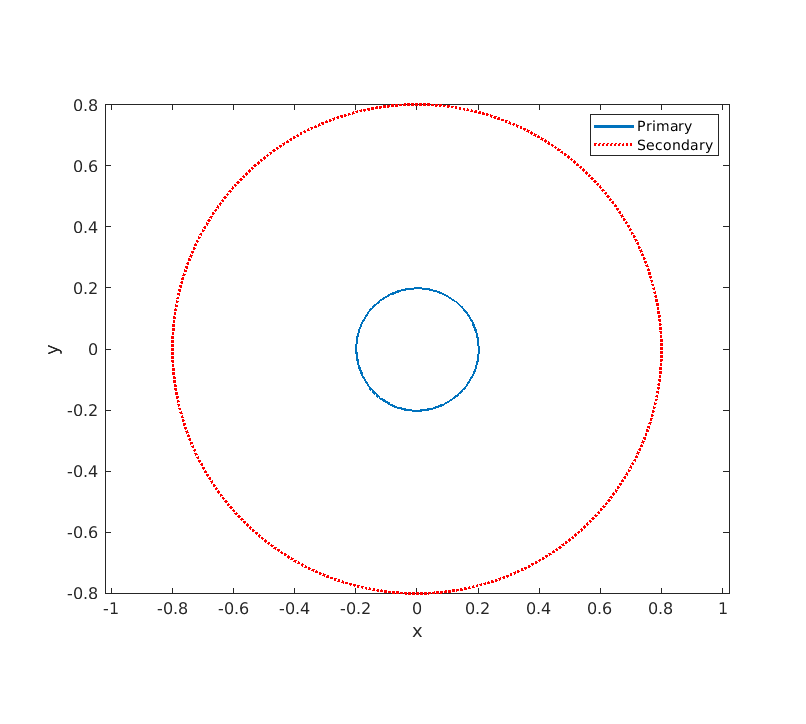
\includegraphics[width=\columnwidth]{../plots/2c_orbits.png}
				\caption{2c}
				\label{fig:2c}
			\end{subfigure}
			\hfill
			\begin{subfigure} {.475\columnwidth}
				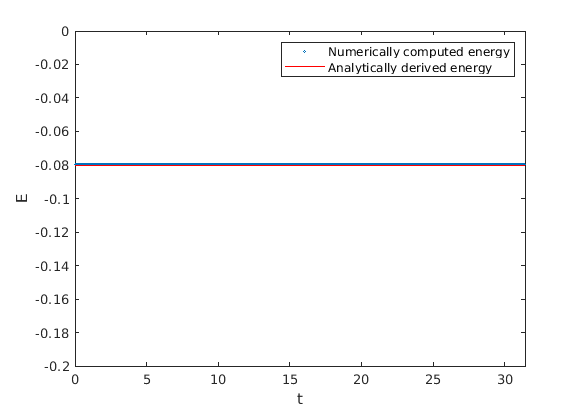
\includegraphics[width=\columnwidth]{../plots/2d_energies.png}
				\caption{2d}
				\label{fig:2d}
			\end{subfigure}
			\caption{Problem 2}
			\label{fig:2}
		\end{figure}
	
		\begin{enumerate} [label*=\textbf{(\alph*)}]
			
			% ---------------------------------- (a) ---------------------------------------------
			
			\item
				\subitem \textbf{Methods  --}
				\subitem \textbf{Results  --}
				\subitem \textbf{Discussions  --}
				
			% ---------------------------------- (b) ---------------------------------------------
			
			\item
				\subitem \textbf{Methods  --}
				\subitem \textbf{Results  --}
				\subitem \textbf{Discussions  --}
			
			% ---------------------------------- (c) ---------------------------------------------
			
			\item
				\subitem \textbf{Methods  --}
				\subitem \textbf{Results  --}
				\subitem \textbf{Discussions  --}
			
			% ---------------------------------- (d) ---------------------------------------------
			
			\item
				\subitem \textbf{Methods  --}
				\subitem \textbf{Results  --}
				\subitem \textbf{Discussions  --}
			
		\end{enumerate}
		
		\lstinputlisting[caption=first code, label=code:2.1,
						firstline=7,firstnumber=9,
						lastline=19]{../problem2/binary.m}
		\lstinputlisting[caption=second code, label=code2.2,
						firstline=4]{../problem2/energyplot.m}


		% -------------------------------- Conclusions --------------------------------------

		\section{Conclusions} \label{2:conclusions}


	% ========================= Problem 3 ===================================================
	
	\clearpage
	\setcounter{section}{0}
	\part{Hypervelocity Stars} \label{Problem3}

		% ------------------------------- Introduction --------------------------------------

		\section{Introduction} \label{3:introduction}

		% -------------------------------- Methods, Results ----------------------------------
		
		\section{Methods, Results and Discussions}
		
			
			\begin{figure} [h]
				\begin{subfigure} {.5\columnwidth}
					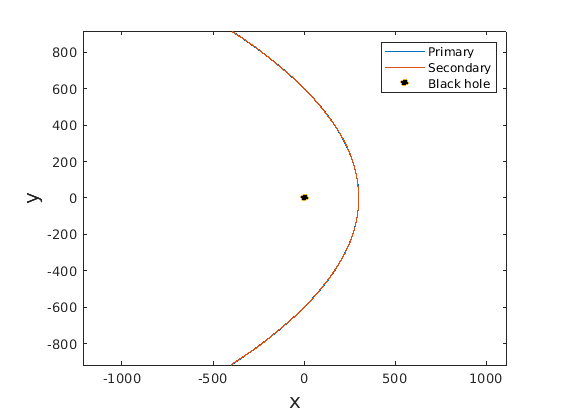
\includegraphics[width=\columnwidth]{../plots/3a_orbits_equalaxes.png}
					\caption{3a}
					\label{fig:3a}
				\end{subfigure}
				\hfill
				\begin{subfigure} {.5\columnwidth}
					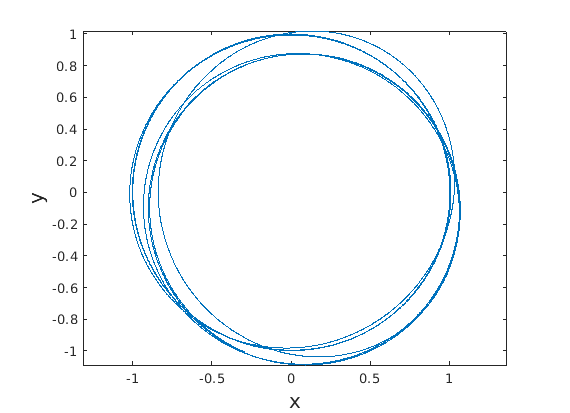
\includegraphics[width=\columnwidth]{../plots/3b_secondaryorbit.png}
					\caption{3b}
					\label{fig:3b}
				\end{subfigure}\\
				
				\begin{subfigure} {\columnwidth}
					\centering
					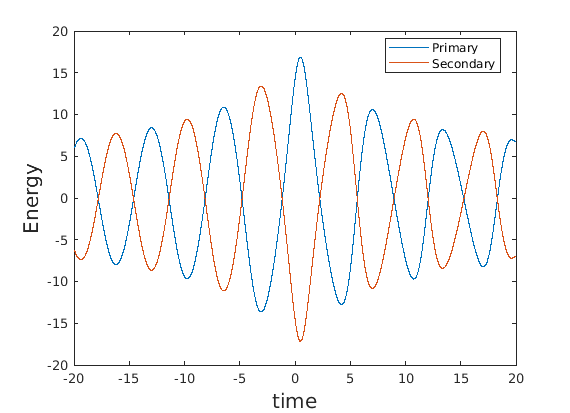
\includegraphics[width=.5\columnwidth]{../plots/3c_energy.png}
					\caption{3c}
					\label{fig:3c}
				\end{subfigure}
				\caption{Problem 3 - fig 1}
				\label{fig:3.1}
			\end{figure}
			
			\begin{figure}
				\begin{subfigure} {.5\columnwidth}
					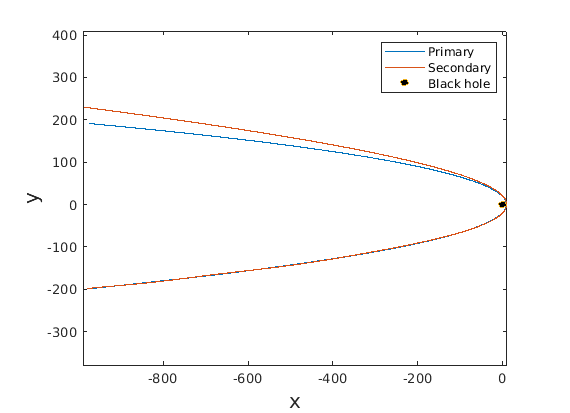
\includegraphics[width=\columnwidth]{../plots/3d_orbitsdisruption_equalaxes.png}
					\caption{3da}
					\label{fig:3da}
				\end{subfigure}
				\hfill
				\begin{subfigure} {.5\columnwidth}
					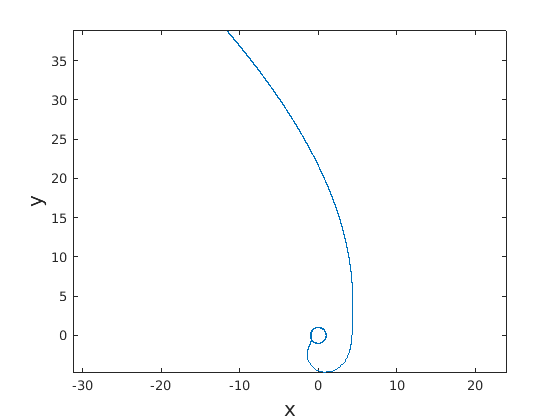
\includegraphics[width=\columnwidth]{../plots/3d_secondaryorbitdisruption_equalaxes.png}
					\caption{3db}
					\label{fig:3db}
				\end{subfigure}\\
				
				\begin{subfigure} {\columnwidth}
					\centering
					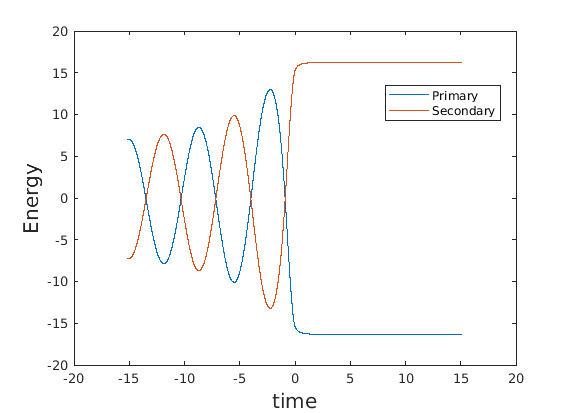
\includegraphics[width=.5\columnwidth]{../plots/3d_energy.png}
					\caption{3dc}
					\label{fig:3dc}
				\end{subfigure}
				\caption{Problem 3 - fig 2}
				\label{fig:3.2}
			\end{figure}
			
			\begin{table}
				\centering
				\begin{tabular} {l l r r}
					\toprule
					\textbf{Quantity} & \textbf{Variable} & \textbf{D=3} & \textbf{D=0.1}\\
					\midrule
					\(t^{}_{0}\) & \texttt{t} & -19.9555 & -15.1290 \\
					\(x^{}_{p}\) & \texttt{x(1)}& -400.0000 & -980.0000 \\
					\(y^{}_{p}\) & \texttt{x(2)} & -917.3151 & -199.7975 \\
					\(v^{}_{px}\) & \texttt{x(3)} & 37.6166 & 44.6972 \\
					\(v^{}_{py}\) & \texttt{x(4)} & 24.4949 & 4.4721 \\
					\(x^{}_{s}\) & \texttt{x(5)} & -400.0000 & -980.0000 \\
					\(y^{}_{s}\) & \texttt{x(6)} & -916.3151 & -198.7975 \\
					\(v^{}_{sx}\) & \texttt{x(7)} & 36.6166 & 43.6972 \\
					\(v^{}_{sy}\) & \texttt{x(8)} & 24.4949 & 4.4721 \\
					\bottomrule
				\end{tabular}
				\caption{Table of variable values for two values of D}
				\label{table:dvalues}
			\end{table}
			
			\lstinputlisting[caption=code 1, label=code:3.initialc,
			firstline=5]{../problem3d/initialc.m}
			\lstinputlisting[caption=code 2, label=code:3.f]{../problem3d/f.m}
			
			
			\begin{enumerate} [label*=\textbf{(\alph*)}]
	
			% ---------------------------------- (a) ---------------------------------------------
	
				\item
					\subitem \textbf{Methods  --}
					\subitem \textbf{Results  --}
					\subitem \textbf{Discussions  --}
	
			% ---------------------------------- (b) ---------------------------------------------
	
				\item
					\subitem \textbf{Methods  --}
					\subitem \textbf{Results  --}
					\subitem \textbf{Discussions  --}
	
			% ---------------------------------- (c) ---------------------------------------------
	
				\item
					\subitem \textbf{Methods  --}
					\subitem \textbf{Results  --}
					\subitem \textbf{Discussions  --}
	
			% ---------------------------------- (d) ---------------------------------------------
	
				\item
					\subitem \textbf{Methods  --}
					\subitem \textbf{Results  --}
					\subitem \textbf{Discussions  --}
	
			\end{enumerate}


		% -------------------------------- Conclusions --------------------------------------

		\section{Conclusions} \label{3:conclusions}



\end{document}